\documentclass[11pt, a4paper]{book}
\usepackage{hyperref}
\usepackage{zref-xr}
\usepackage{zref-clever}
\zexternaldocument{main}

\ExplSyntaxOn
%* Here we want to extract all labels in \jobname.aux (where \jobname.tex should be a homework-type file.). Then, we undefine these labels from \zexternaldocument{main} so that unwanted warnings of multiply defined labels don't haunt us --- when main.aux and \jobname.aux share common labels --- while still allowing us to check for actual multiply defined labels inside \jobname.aux. 
    % Label extraction
        % New variables
            % The sequence of all labels in \jobname.aux
            \seq_new:N \g__Prassble_all_labels_seq
            % The io-read stream we want to use
            \ior_new:N \l__Prassble_hw_aux_ior
        % Open the stream \jobname.aux 
        \ior_open:Nn \l__Prassble_hw_aux_ior {\jobname.aux}
        \ior_map_inline:Nn \l__Prassble_hw_aux_ior 
        {
            % If \newlabel{ <label name> }... is present, extract <label name> under the second item of the sequence \t_tmpa_seq. Otherwise, do nothing.
            \regex_extract_once:nnN 
            { \c{newlabel} \cB. (\c[^BE].*) \cE. } 
            { #1 }
            \l_tmpa_seq
            % Store the <label name> inside the sequence \g__Prassble_all_labels_seq of all labels in \jobname.aux.
            \seq_gput_right:Ne \g__Prassble_all_labels_seq { \seq_item:Nn \l_tmpa_seq { 2 } }
        }
        % We are done with reading \jobname.aux, so we close the corresponding ior stream.
        \ior_close:N \l__Prassble_hw_aux_ior
        % Remove all empty items from the sequence \g__Prassble_all_labels_seq of all labels in \jobname.aux.
        \seq_gremove_all:Nn \g__Prassble_all_labels_seq {}
    % Undefine external labels
    \seq_map_inline:Nn \g__Prassble_all_labels_seq {\cs_undefine:c{Z@R@#1}}
\ExplSyntaxOff

\begin{document}
\section{Homework \#1}
This external reference is fine: \zcref{fig:main}. The warning about the label \verb|fig:1| being multiply defined is issued: \zcref{fig:1}
\newpage
\begin{definition}
    This is the first definition of the first homework.
\end{definition}
\begin{exercise}[label=ex:H.1.1]
    This is the first exercise of the first homework.
\end{exercise}
\begin{proof}
    This is the first proof of the first exercise of the first homework. We can easily reference labels from \codeinline{text}{main.tex}, e.g. \zcref{thm:1.1}.
\end{proof}

\begin{exercise}[label=ex:H.1.2]
    This is the second exercise of the first homework.
\end{exercise}
\begin{proof}
    This is the first proof of the second exercise of the first homework. We reference \zcref{ex:H.1.1} here.
\end{proof}

\begin{exercise}[label=ex:H.1.3]
    This is the third exercise of the first homework.
\end{exercise}
\begin{answer}
    The answer to \zcref{ex:H.1.3}
\end{answer}

We insert \zcref{fig:Three_Plane_Orthogonal_Complements} as an example figure:
\begin{figure}[H]
    \centering
    \includegraphics[page=2]{Three_Planes_Orthogonal_Complements_licensed_under_CC_BY-SA_4.0.pdf}
    \caption{A figure whose author \extref{https://github.com/GrassGlass}{Grass} licenses under \extref{https://creativecommons.org/licenses/by-sa/4.0/}{CC BY-SA 4.0}.}
    \label{fig:Three_Plane_Orthogonal_Complements}
\end{figure}
% %* Uncomment this to see that label warnings still function
% \begin{figure}[htbp]
%     \centering
%     \caption{A duplicate of the label \texttt{fig:1} which should cause a warning.}
%     \label{fig:1}
% \end{figure}
\end{document}